\documentclass[compress,mathserif,fleqn,10pt]{beamer}
\useoutertheme{split}
\useoutertheme[subsection=false]{smoothbars}
\useinnertheme[shadow=true]{rounded}
\usecolortheme{whale}
\usecolortheme{orchid}

\setbeamerfont{block title}{size={}}
\setbeamertemplate{navigation symbols}{}
\beamersetuncovermixins{\opaqueness<1->{15}}{}
% \setbeamertemplate{page number in head/foot}[totalframenumber]

\makeatletter
\let\beamer@writeslidentry@miniframeson=\beamer@writeslidentry%
\def\beamer@writeslidentry@miniframesoff{%
	\expandafter\beamer@ifempty\expandafter{\beamer@framestartpage}{}% does not happen normally
	{%else
		% removed \addtocontents commands
		\clearpage\beamer@notesactions%
	}
}
\newcommand*{\miniframeson}{\let\beamer@writeslidentry=\beamer@writeslidentry@miniframeson}
\newcommand*{\miniframesoff}{\let\beamer@writeslidentry=\beamer@writeslidentry@miniframesoff}
\makeatother

\setlength{\mathindent}{0.5cm}
\setcounter{tocdepth}{2}

\usepackage[utf8]{inputenc}
\usepackage{amsmath}
\usepackage{color}
\usepackage{hhline}
\usepackage{epstopdf}
\usepackage{animate}
\usepackage{textpos}
\usepackage{enumerate}
\usepackage{tikz}

\title{Transformers and Multi-features Time2Vec for Financial Prediction}
\author[Bui Nguyen Kim Hai, Nguyen Duy Chien]{Bui Nguyen Kim Hai, Nguyen Duy Chien}
%\institute{Department of Numerical Analysis, Faculty of Informatics\\ ELTE Eötvös Loránd University, Budapest, Hungary}
\date{\scriptsize \emph{TDK CONFERENCE – IT SCIENCE SECTION, 2024 SPRING}\\\bigskip Budapest, Hungary\\ May 29, 2024}

\begin{document}
	
	\abovedisplayskip=1pt
	\belowdisplayskip=2pt
	\abovedisplayshortskip=1pt
	\belowdisplayshortskip=2pt
	
	\begin{frame}
		\titlepage
	\end{frame}
	
	\begin{frame}\frametitle{Outline}
		\tableofcontents
	\end{frame}
	
	\section{Introduction}
	\begin{frame}\frametitle{Outline}
		\tableofcontents[currentsection]
	\end{frame}
	
	\subsection{Motivation}
	\begin{frame}{Motivation}
		\begin{block}{By other works}
			\begin{itemize}
				\item Researchers try to combine Time2Vec with CNN, RNN, LSTM, and Attention mechanism
				\item For instances:
				
					\begin{itemize}
						\item Aeroengine Risk Assessment
						\item Predicting Production in Shale and Sandstone Gas Reservoirs
						\item Stock Price Forecasting
					\end{itemize}
			\end{itemize}
		\end{block}
		\smallskip
		\begin{block}{In finance area}
			\begin{itemize}
				\item Studies primarily rely on one dataset
			\end{itemize}
		\end{block}
		\smallskip
		\begin{block}{By observing trends}
			\begin{itemize}
				\item Stock's trend is a Markov process
				\item Historical data offers limited foresight
				\item Stocks having similar trend is more promising
			\end{itemize}
		\end{block}
	\end{frame}
	
	\begin{frame}{Motivation: Cross-correlation to NASDAQ}
		\centerline{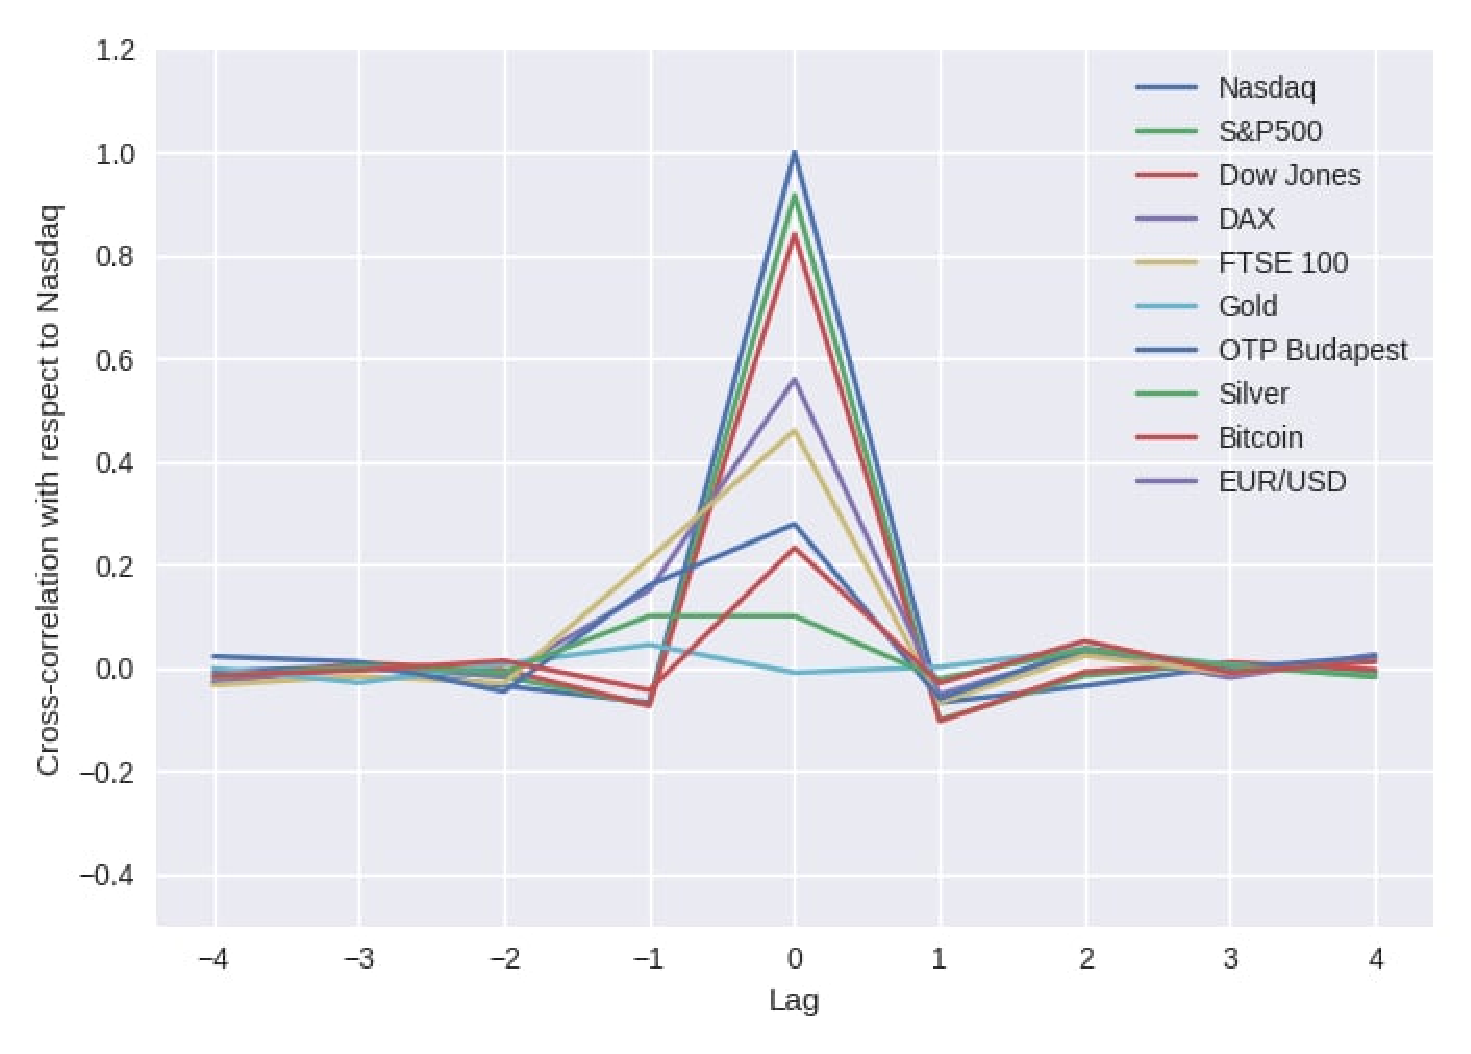
\includegraphics[width=0.85\textwidth]{images/nas_base.eps}}
	\end{frame}

	\begin{frame}{Motivation: Cross-correlation to Exxon Mobil}
		\centerline{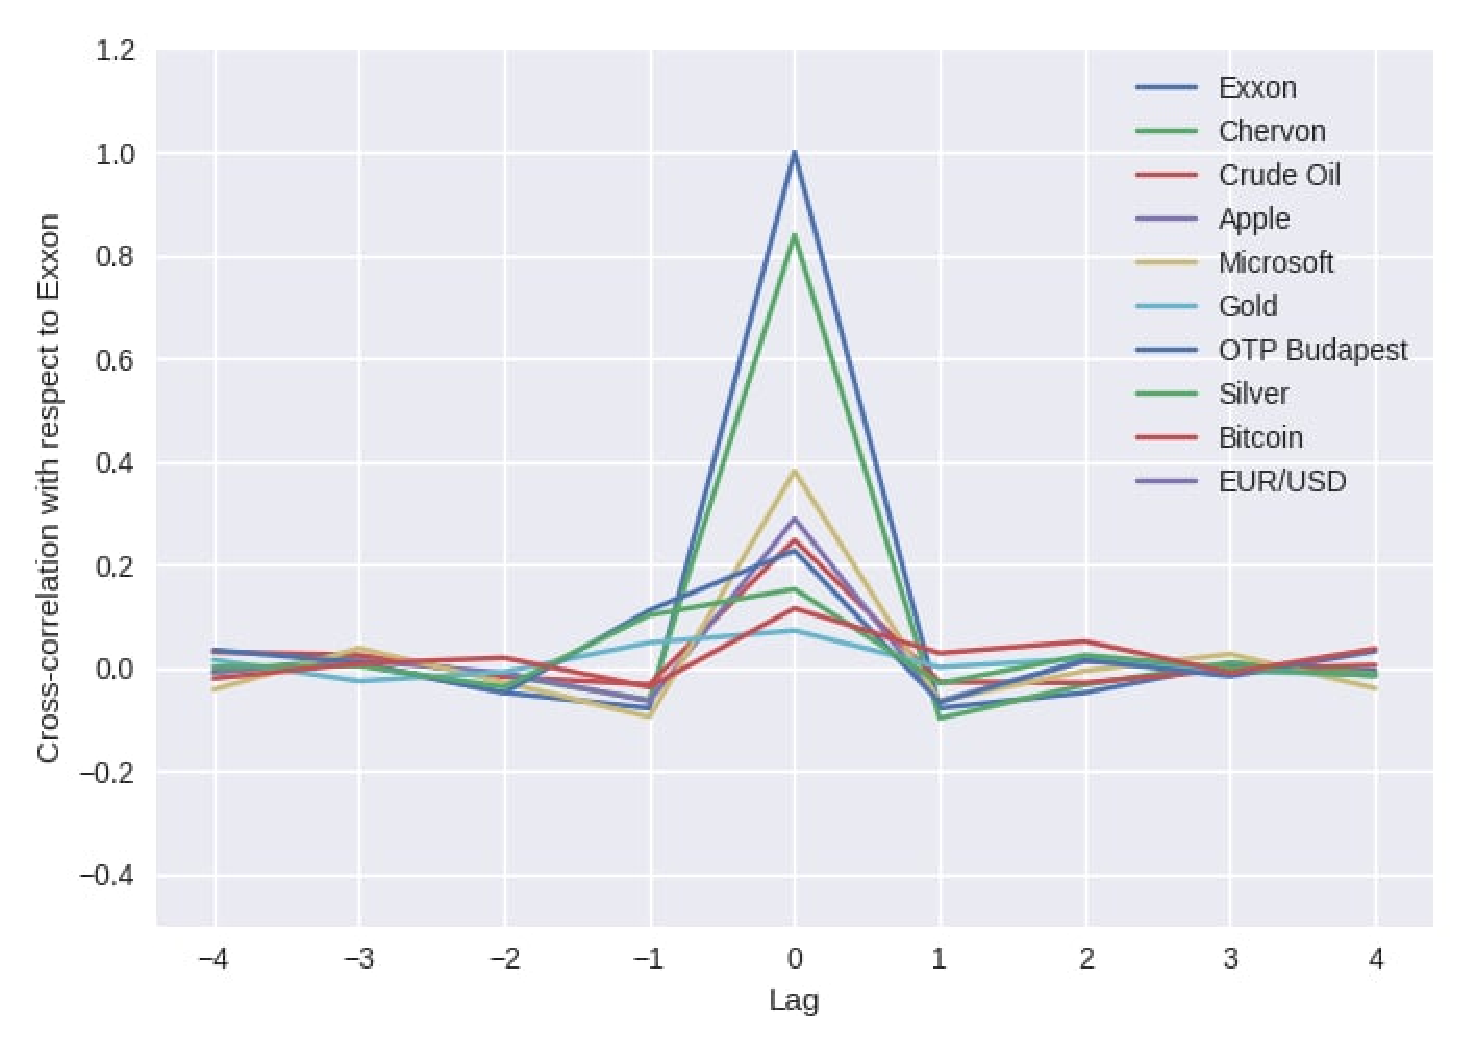
\includegraphics[width=0.85\textwidth]{images/exx_base.eps}}
	\end{frame}
	
	\subsection{Related work}
	\begin{frame}{Related work}
		\begin{block}{ARIMA}
			Making one-step-ahead predictions
		\end{block}
		\begin{block}{RNN}
			Handling temporal problems in sequential data and time-series analysis.
		\end{block}
		\begin{block}{LSTM}
			Using gates, LSTM enables network to learn long-term dependencies and prevent the vanishing gradient problem.
		\end{block}
		\begin{block}{Transformer}
			The SOTA architecture that works well in many area such as NLP, and time-series 
		\end{block}
		\begin{block}{Time2Vec}
			Use to embed the time-series data to vector
		\end{block}
	\end{frame}
	
	\section{Proposed model and techniques}
	\begin{frame}\frametitle{Outline}
		\tableofcontents[currentsection]
	\end{frame}
	
	%\subsection{Behavioral similarity of stocks}
	%\begin{frame}{Behavioral similarity of stocks}
		
	%\end{frame}
	
	\subsection{Data collection}
	\begin{frame}{Data collection}
		\begin{exampleblock}{Where to collect?}
			Yahoo Finance
		\end{exampleblock}
		\begin{exampleblock}{What will be collected?}
			Date, Open, High, Low, Close, Volume columns
		\end{exampleblock}
		\begin{exampleblock}{How many datasets should we collect?}
			Two, three, four ..., as long as they are highly correlated to each other
		\end{exampleblock}
		\begin{block}{Collected datasets}
			\begin{itemize}
				\item \structure{Group1}: NASDAQ, S\&P500, DJI, DAX
				\item \structure{Group2}: Exxon Mobil, Chervon
			\end{itemize}
		\end{block}
	\end{frame}
	
	\subsection{Preprocessing data}
	\begin{frame}{Preprocessing data: The pipeline}
		\centerline{\includegraphics[width=0.8\paperwidth]{images/pipeline-big.eps}}
		\centerline{The preprocessing data pipeline.}
		\begin{block}{Techniques}
			\begin{itemize}
				\item \structure{Fill-forward}: Filling missing data in dataset
				\item \structure{Moving Average}: Smoothing dataset by averaging data
				\item \structure{Percentage Change}: Compute the difference in the data
				\item \structure{Min-Max Normalization}: Normalizing dataset
				\item \structure{Geometry Mean Not NaN (GMNN)}: Combining multiple datasets
			\end{itemize}
		\end{block}
	\end{frame}
	
	\begin{frame}{Preprocessing data: But... What is GMNN?}
		\begin{columns}
			\begin{column}{0.5\textwidth}
				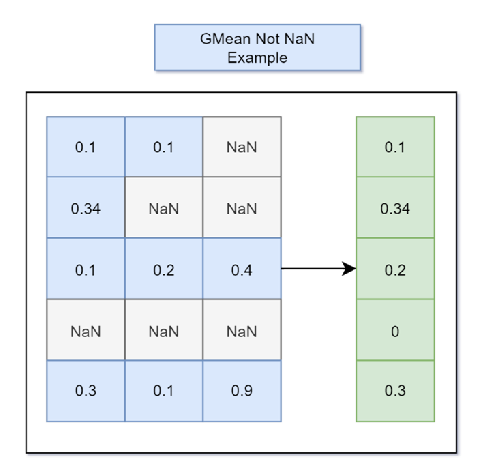
\includegraphics[width=\textwidth]{images/gmnn.eps}
			\end{column}
			\begin{column}{0.5\textwidth}
				\begin{block}{GMNN Attributes}
					\begin{itemize}
						\item \structure{Union}: Handling length difference when combining datasets
						\smallskip
						\item \structure{Invariant}: Keeping the data stays normalized
						\smallskip
						
						\item \structure{Representation}: The output reflects the whole datasets
						\smallskip
						
					\end{itemize}
				\end{block}
				\vspace*{1cm}
			\end{column}
		\end{columns}
		\bigskip
		\centerline{A simple sample of applying GMNN transformation}
	\end{frame}
	
	\subsection{Model architecture}
	\begin{frame}{Model architecture: Proposed model}
		\begin{columns}
			\begin{column}{0.45\textwidth}
				\centerline{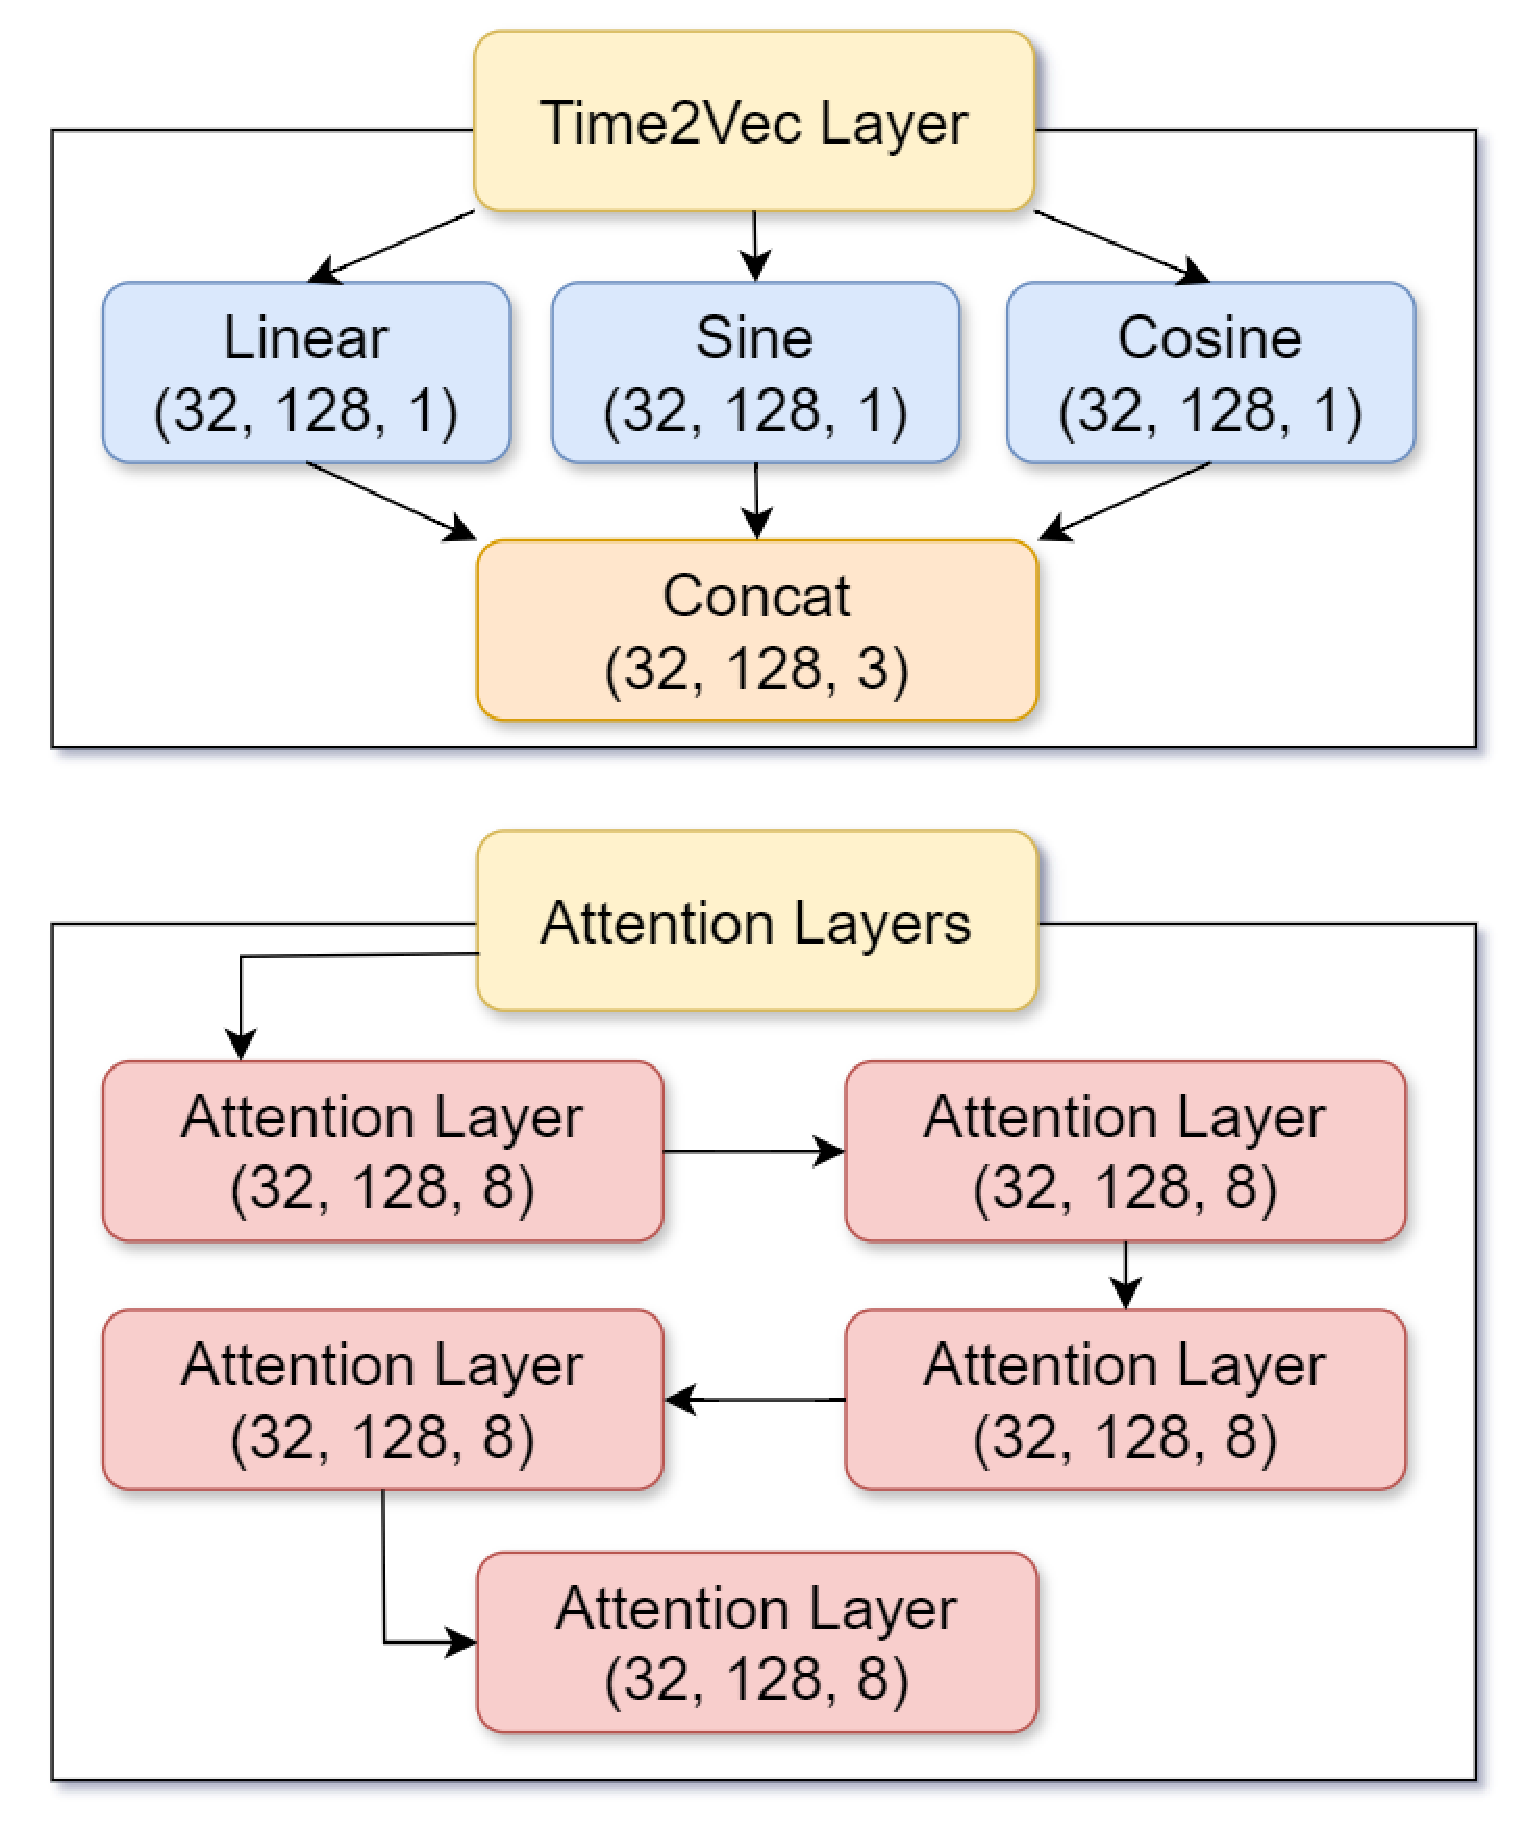
\includegraphics[width=\textwidth]{images/model-parts.eps}}
			\end{column}
			\begin{column}{0.45\textwidth}
				\centerline{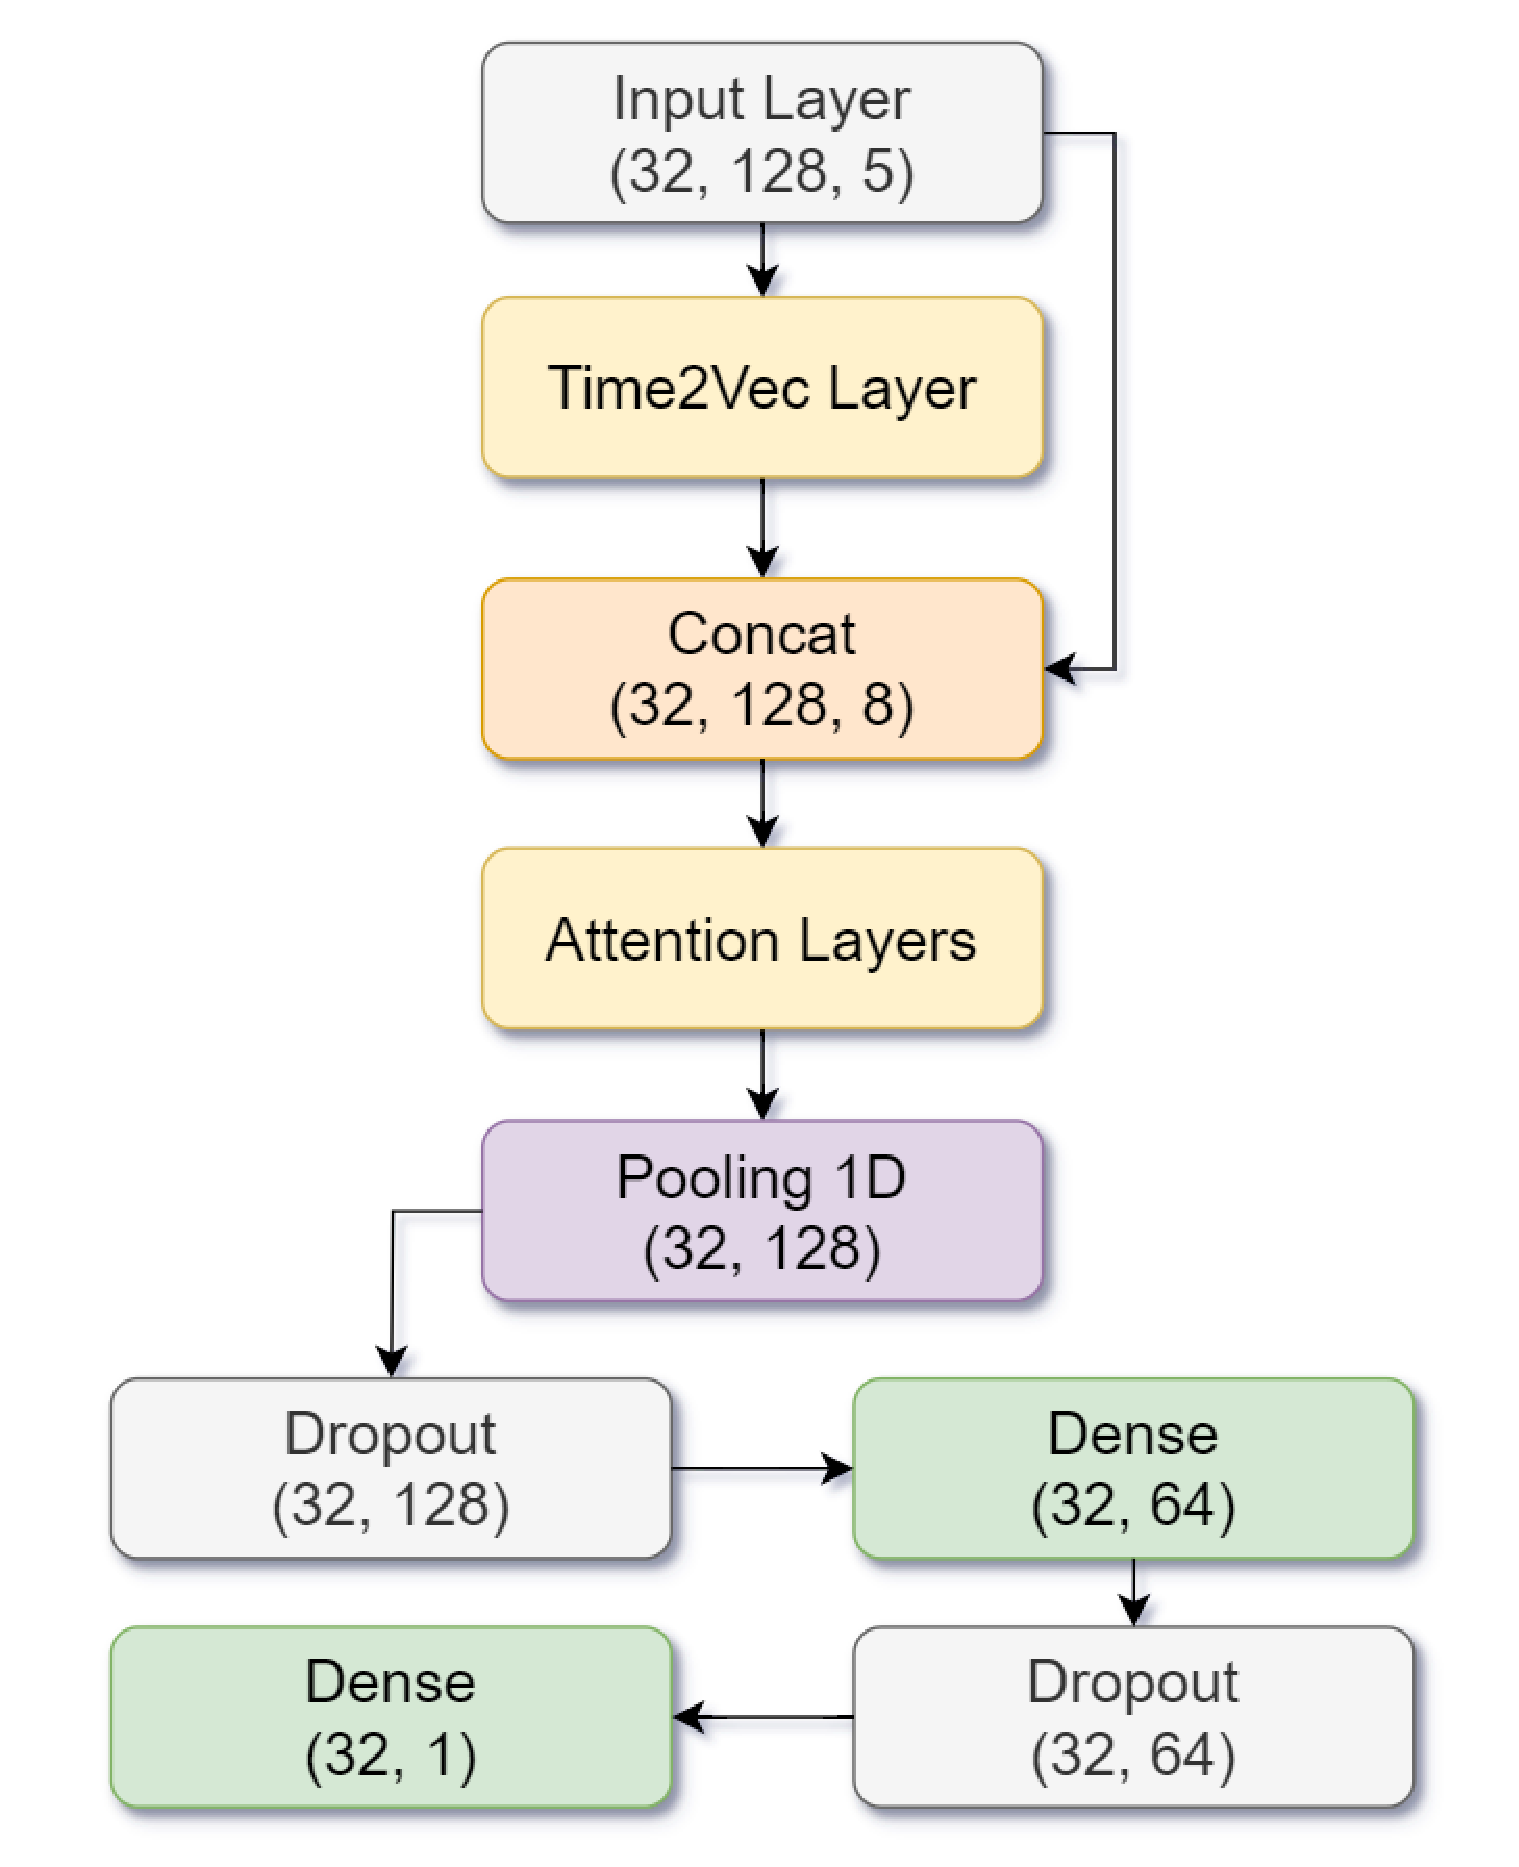
\includegraphics[width=\textwidth]{images/model-mini.eps}}
			\end{column}
		\end{columns}
	\end{frame}
	
	\begin{frame}{Model architecture: Role of layers}
		\begin{columns}
			\begin{column}{0.45\textwidth}
				\centerline{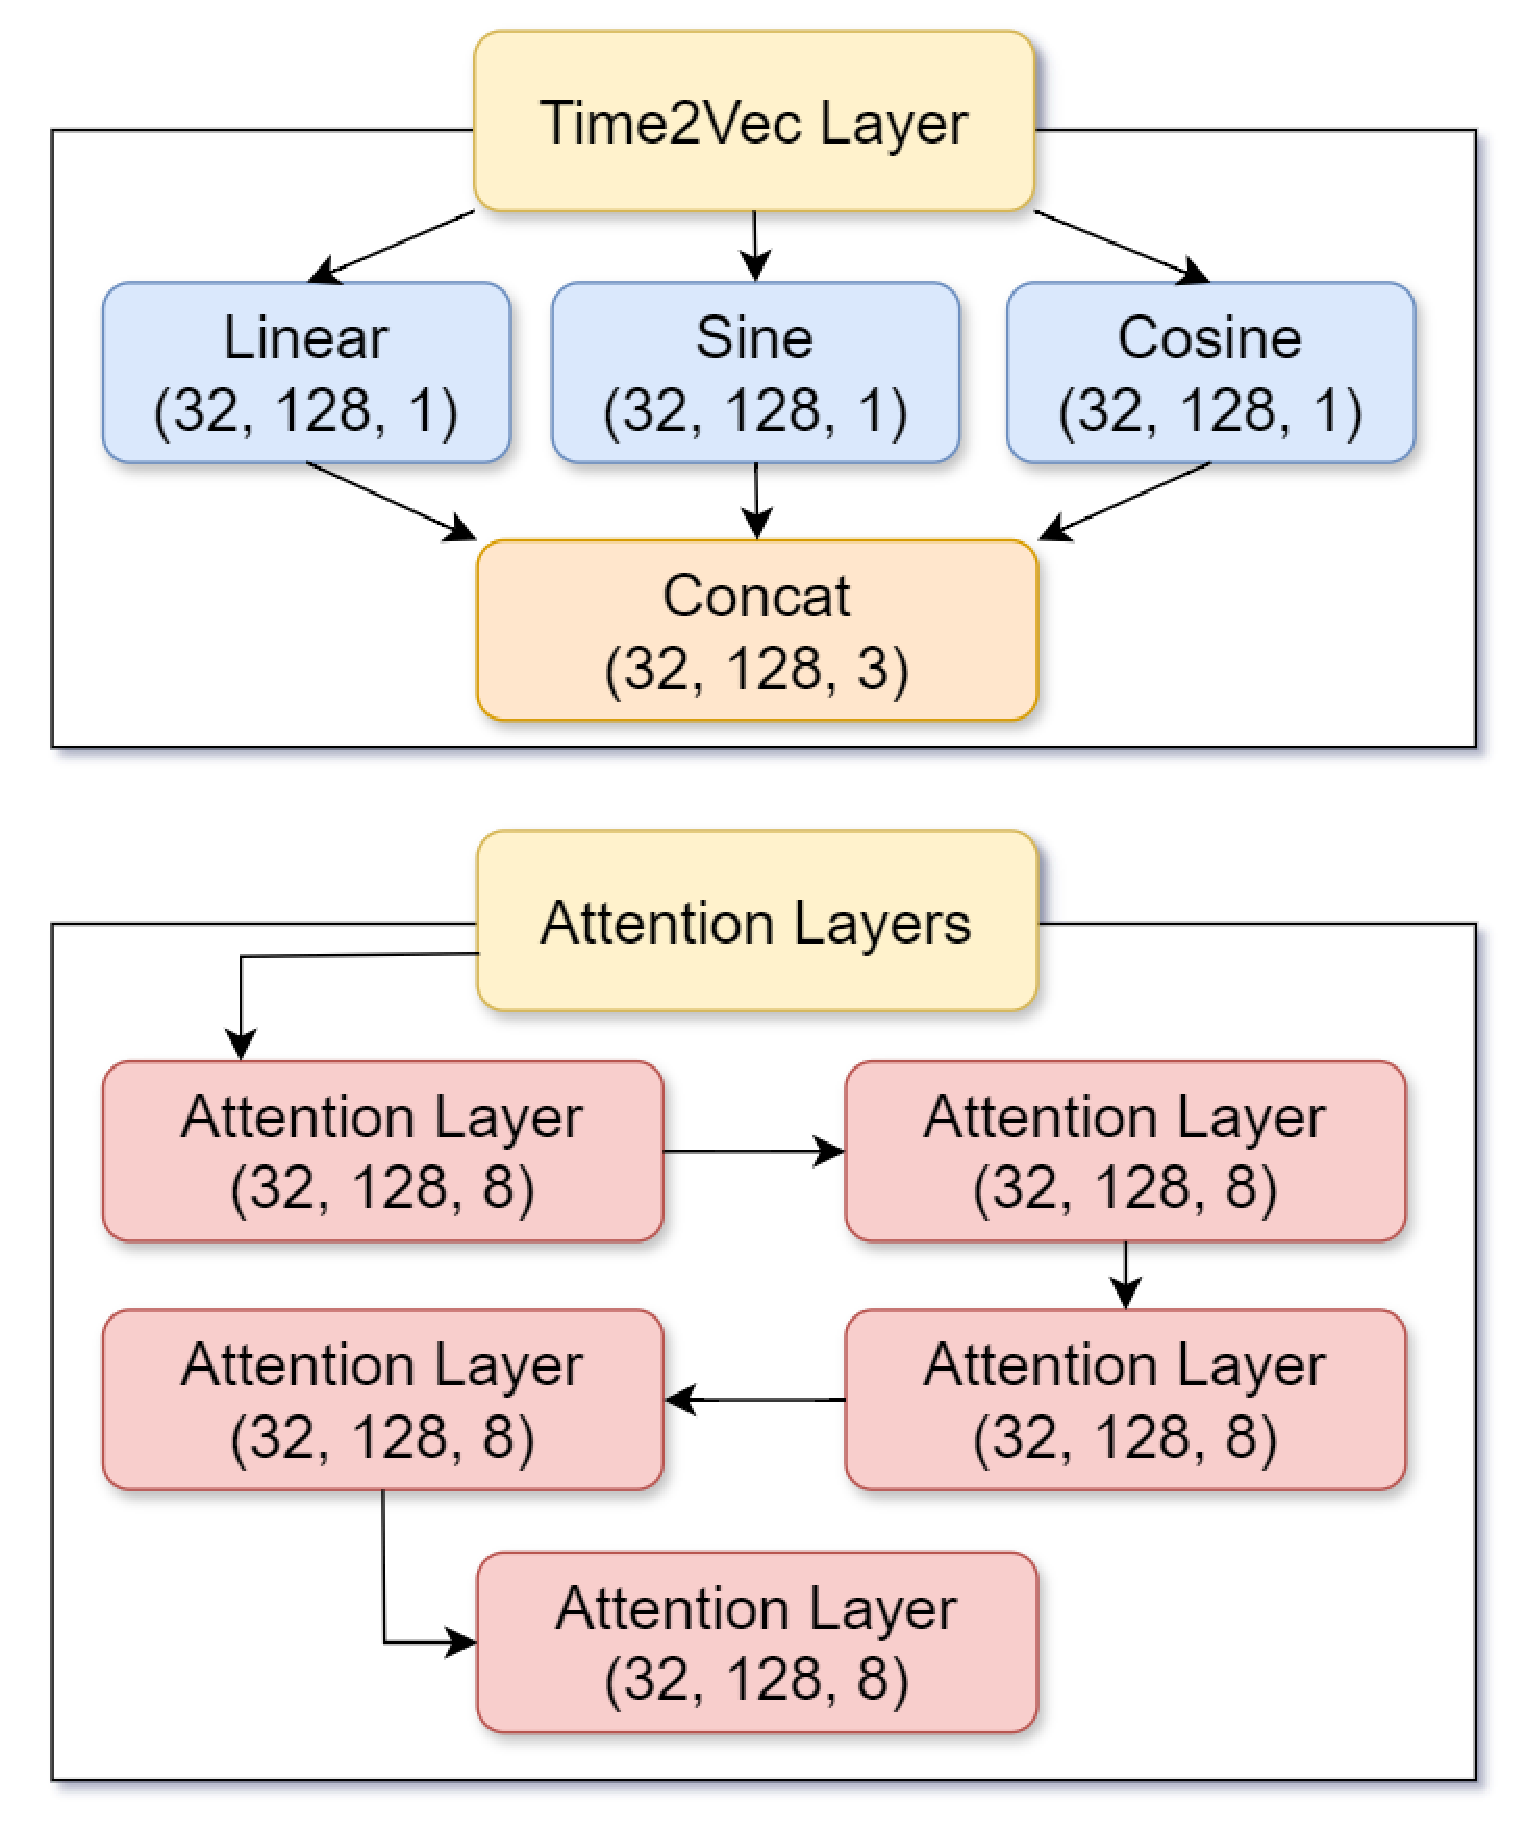
\includegraphics[width=\textwidth]{images/model-parts.eps}}
			\end{column}
			\begin{column}{0.55\textwidth}
				\begin{block}{Roles}
					\begin{itemize}
						\item \structure{Time2Vec}
							\begin{itemize}
								\item \structure{Linear}: Capturing linear trends \smallskip
								\item \structure{Sine, Cosine}: Encoding positions and capturing periodic behaviors \smallskip
								\item \structure{Concat}: Concatenating above three layers 
							\end{itemize}
						\bigskip
						\item \structure{Attention Layers}
							\begin{itemize}
								\item To study the trend from different aspects, positions \smallskip
							\end{itemize}
					\end{itemize}
				\end{block}
			\end{column}
		\end{columns}
	\end{frame}
	
	\begin{frame}{Model architecture: Role of layers}
		\begin{columns}
			\begin{column}{0.55\textwidth}
				\begin{block}{Roles}
					\begin{itemize}
						\item \structure{Time2Vec}: Catch continuous attribute of time
						\item \structure{Concat}: Apply Residual Connection
						\item \structure{Attention}: Deep understanding trend movements
						\item \structure{Pooling}: Reducing dimension
						\item \structure{Dropout}: Prevent over-fitting
						\item \structure{Dense}: Apply activation functions (ReLU)
					\end{itemize}
				\end{block}
			\end{column}
			\begin{column}{0.45\textwidth}
				\centerline{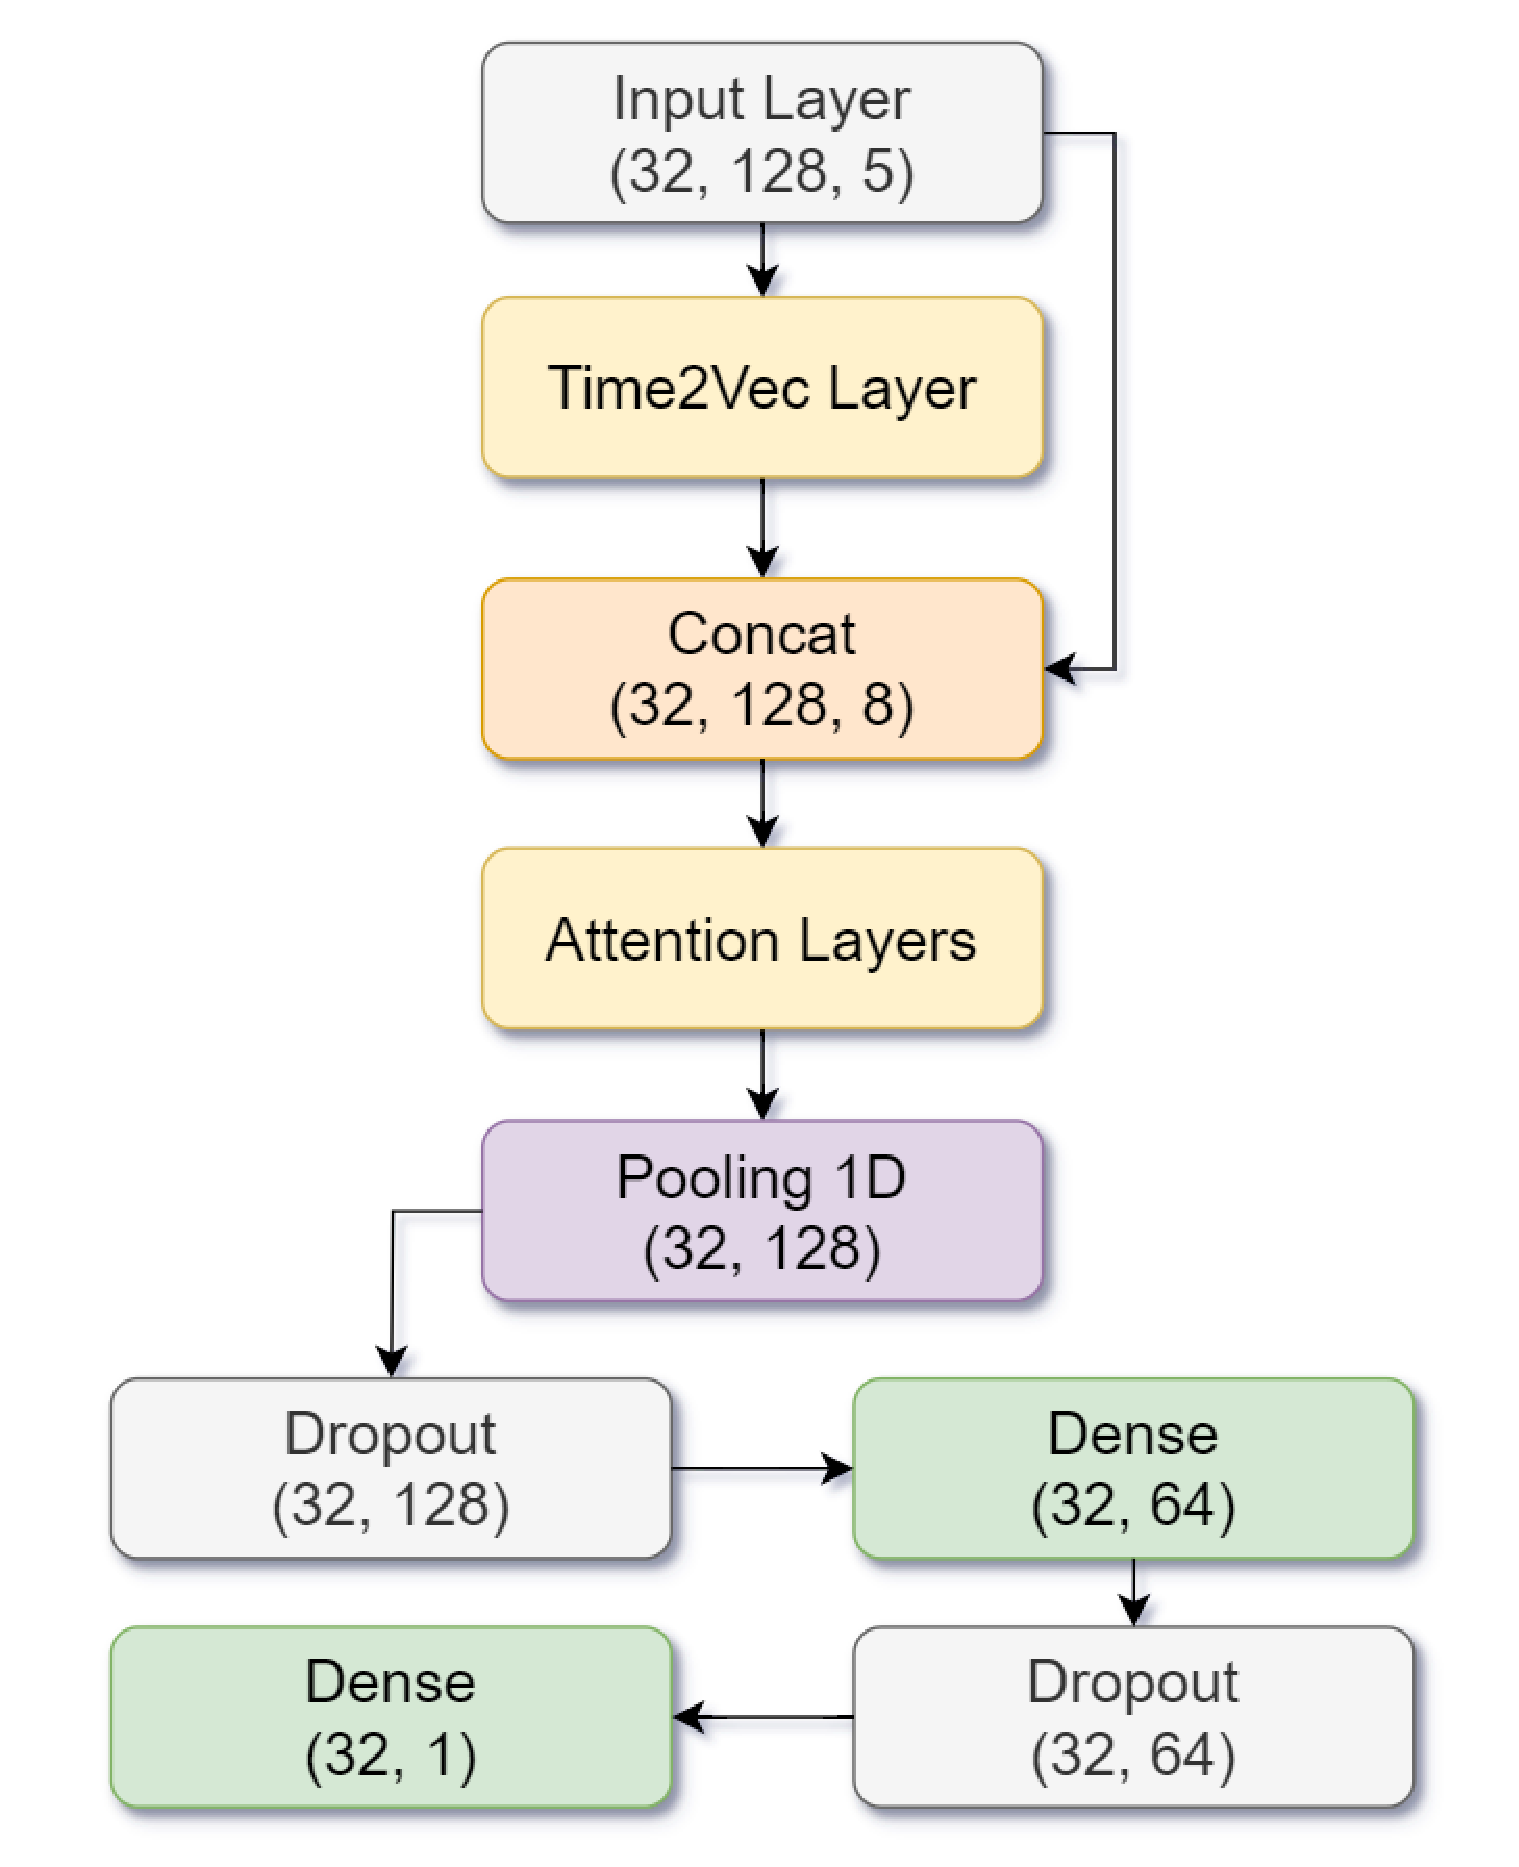
\includegraphics[width=\textwidth]{images/model-mini.eps}}
			\end{column}
		\end{columns}
	\end{frame}
	
	\subsection{Decoding engineering}
	\begin{frame}{Decoding engineering}
		\centerline{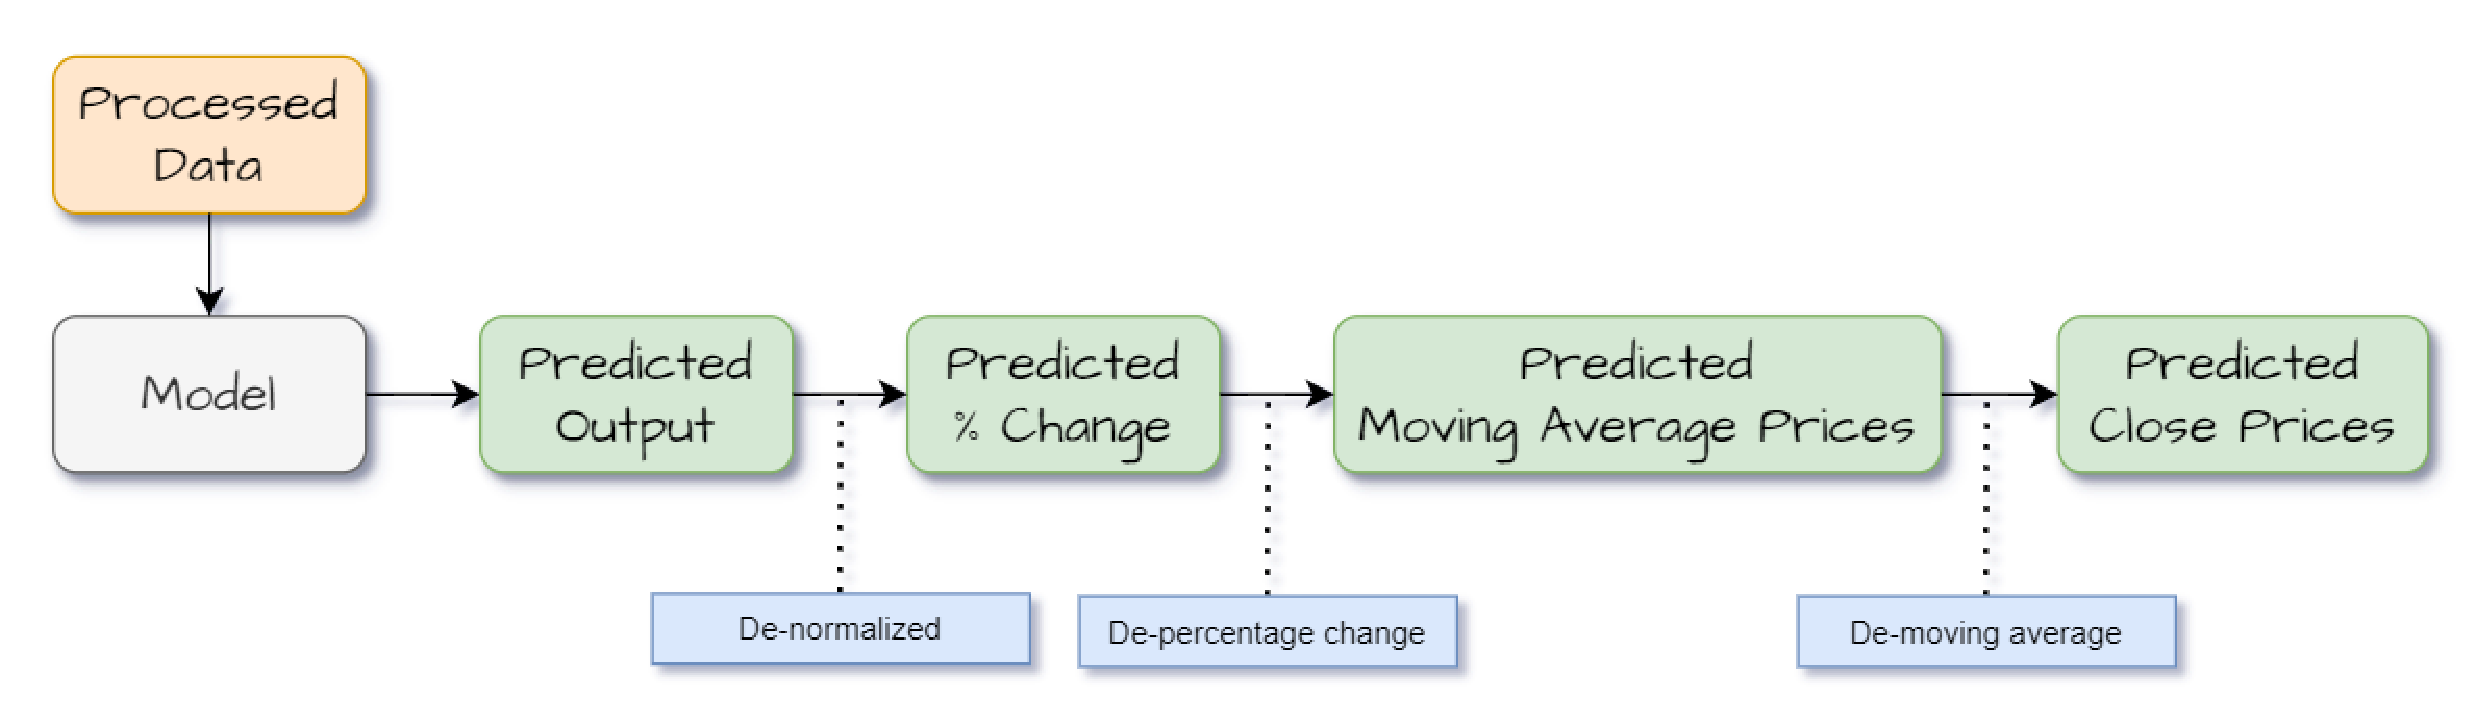
\includegraphics[width=0.8\paperwidth]{images/decode.eps}}
		\centerline{The decoding pipeline.}
		\begin{columns}
			\begin{column}{0.5\textwidth}
				\begin{block}{Techniques}
					\begin{minipage}[t][2cm][t]{\textwidth}
						\begin{itemize}
							\item De-normalized
							\item De-percentage change
							\item De-moving average
						\end{itemize}
					\end{minipage}
				\end{block}
			\end{column}
			\begin{column}{0.5\textwidth}
				\begin{exampleblock}{Why don't we use De-GMNN step?}
					\begin{minipage}[t][2cm][t]{\textwidth}
						\begin{itemize}
							\item Output is \textbf{normalized} (Invariant)
							\item Target is \textbf{one} dataset, output only reflects that one
						\end{itemize}
					\end{minipage}
				\end{exampleblock}
			\end{column}
		\end{columns}
	\end{frame}
	
	\section{Results and Conclusion}
	\begin{frame}{Outline}
		\tableofcontents[currentsection]
	\end{frame}
	
	\begin{frame}{Results}
		\begin{columns}
			\begin{column}{0.5\textwidth}
				\centerline{\includegraphics[width=1.12\textwidth]{images/exxon-big.eps}}
			\end{column}
			\begin{column}{0.5\textwidth}
				\centerline{\includegraphics[width=1.12\textwidth]{images/nasdaq-big.eps}}
			\end{column}
		\end{columns}
		
		\smallskip
		\centerline{Comparing 6 metrics with respect to Exxon (Left), NASDAQ (Right)}
	\end{frame}
	
	\begin{frame}\frametitle{Conclusion}
		\begin{block}{Conclusion}
			\smallskip
			By leveraging multiple criteria to evaluate the proposed model such as
			\begin{itemize}
				\item MAE, MAPE, RMSE, MSE, R2-score (price prediction task)
				\smallskip
				\item Accuracy (trend forecasting task)
			\end{itemize}
			 \bigskip
			 
			 We can proudly say that, the multi-feature model
			 \begin{itemize}
			 	\item \textbf{Outperforms} the single-feature one in most cases and they are \textbf{extremely close} to each other in other scenarios.
			 	\smallskip
			 	\item Usually yields \textbf{better} result than the SOTA in almost every contexts.
			 \end{itemize}
			 \smallskip
		\end{block}
	\end{frame}
	
	\section{Summary}
	\begin{frame}\frametitle{Outline}
		\tableofcontents[currentsection]
	\end{frame}
	
	\begin{frame}{Summary}
		\begin{exampleblock}{Summary}
			\begin{itemize}
				\item We explore deep learning for challenging stock price prediction
				\item Paving the way for new feature studies and applications in various deep learning models
				\item Demonstrates correlation-based features and innovative neural networks improve stock
				price prediction
			\end{itemize}
		\end{exampleblock}
		
		\begin{block}{Further Research}
			\begin{itemize}
				\item Fine-tuning the architecture
				\item Continuing improving processing methods
				\item Comparing to other SOTA neural networks like KAN
				\item Applying the architecture to other areas
			\end{itemize}
		\end{block}
	\end{frame}
	\miniframesoff
	\section*{}
	\begin{frame}
		\begin{beamercolorbox}[sep=8pt,center,shadow=true,rounded=true]{title}
			\usebeamerfont{title}Thank you for your attention!\par%     
		\end{beamercolorbox}
	\end{frame}
\end{document}